\documentclass[a4paper]{article}

%%%%%%%%%%%%%%%%%%%%%%%%%%%%%%%%%% 
% Package for making LaTeX properly handle utf8 characters set and danish language rules
\usepackage[utf8]{inputenc}
\usepackage[danish]{babel}

%%%%%%%%%%%%%%%%%%%%%%%%%%%%%%%%%% 
% Package for changing to a nicer font 
\usepackage[T1]{fontenc}

%%%%%%%%%%%%%%%%%%%%%%%%%%%%%%%%%% 
% Package for conctroling the text area
\usepackage[margin=2.5cm]{geometry}

%%%%%%%%%%%%%%%%%%%%%%%%%%%%%%%%%% 
% Package for inserting clickable hyperlinks in pdf versions as produced by pdflatex
\usepackage{enumitem, hyperref}

%%%%%%%%%%%%%%%%%%%%%%%%%%%%%%%%%% 
% Package for including figures. TeX and thus LaTeX was developped before the existence of directory file-structures, but the graphicspath let's you add directories, that the \includegraphics will search.
\usepackage{graphicx}
\graphicspath{{figures/}}

%%%%%%%%%%%%%%%%%%%%%%%%%%%%%%%%%% 
% Package for typesetting programs. Listings does not support fsharp, but a little modification goes a long way
\usepackage{listings}
\usepackage{xcolor}
\usepackage{verbatim}
\usepackage{color}

\renewcommand{\figurename}{Figur}
\renewcommand{\contentsname}{Indholdsfortegnelse}
\renewcommand{\contentsname}{Table of Contents}
\renewcommand{\lstlistingname}{Kildekode}
\renewcommand{\partname}{Afsnit}

\def\sectionautorefname~#1\null{%
  Afsnit #1\null
}

\def\subsectionautorefname~#1\null{%
  Afsnit #1\null
}

\def\figureautorefname~#1\null{%
  Figur #1\null
}

\def\equationautorefname~#1\null{%
  Ligning #1\null
}

\def\namedlabel#1#2{\begingroup
    #2%
    \def\@currentlabel{#2}%
    \phantomsection\label{#1}\endgroup
}

\definecolor{bluekeywords}{rgb}{0.13,0.13,1}
\definecolor{greencomments}{rgb}{0,0.5,0}
\definecolor{turqusnumbers}{rgb}{0.17,0.57,0.69}
\definecolor{redstrings}{rgb}{0.5,0,0}
\definecolor{lightgray}{RGB}{240, 240, 240}

\newcommand{\namedref}[1]{\autoref{#1} - \nameref{#1} på Side \pageref{#1}}

\lstdefinelanguage{FSharp}
				{morekeywords={\#load, \#r, let, new, match, with, rec, open, module, namespace, type, of, member, and, for, in, do, begin, end, fun, function, try, mutable, if, then, else, List, Set, Sudoku, Seq, false, true, Assert, printfn, print, sprintf, when, ->, >, ::, printf, yield, this},
	keywordstyle=\color{bluekeywords},
	sensitive=false,
	morecomment=[l][\color{greencomments}]{///},
	morecomment=[l][\color{greencomments}]{//},
	morecomment=[s][\color{greencomments}]{{(*}{*)}},
	morestring=[b]",
	stringstyle=\color{redstrings},
	tabsize=2, % sets default tabsize to 2 spaces
	backgroundcolor=\color{lightgray}
}

\usepackage[table]{}
\usepackage{array}
\usepackage{algorithm}
\usepackage{caption}
\usepackage{float}
\usepackage{amsmath}
\usepackage{algorithm}
\usepackage[noend]{algpseudocode}
\usepackage{mathtools}
\usepackage{ragged2e}
\usepackage{caption}
\usepackage{amssymb}
\usepackage{nameref}
\usepackage{lmodern}
\usepackage{enumitem}

\lstset{ %
  numbers=right,                    % where to put the line-numbers; possible values are (none, left, right)
  numbersep=5pt,                   % how far the line-numbers are from the code
  numberstyle=\small\color{bluekeywords}, % the style that is used for the line-numbers
  stepnumber=1,                    % the step between two line-numbers. If it's 1, each line will be numbered
  title=\lstname,                   % show the filename of files included with \lstinputlisting; also try caption instead of title
  showstringspaces=false,
  breaklines=true,
  captionpos=b,
  language=FSharp,
  texcl=true,
  extendedchars=true,
  inputencoding=utf8
}

\colorlet{punct}{red!60!black}
\definecolor{background}{HTML}{EEEEEE}
\definecolor{delim}{RGB}{20,105,176}
\colorlet{numb}{blue}

\lstdefinelanguage{json}{
    basicstyle=\normalfont\ttfamily,
    numbers=left,
    numberstyle=\scriptsize,
    stepnumber=1,
    numbersep=8pt,
    showstringspaces=false,
    breaklines=true,
    frame=lines,
    backgroundcolor=\color{background},
    literate=
     *{0}{{{\color{numb}0}}}{1}
      {1}{{{\color{numb}1}}}{1}
      {2}{{{\color{numb}2}}}{1}
      {3}{{{\color{numb}3}}}{1}
      {4}{{{\color{numb}4}}}{1}
      {5}{{{\color{numb}5}}}{1}
      {6}{{{\color{numb}6}}}{1}
      {7}{{{\color{numb}7}}}{1}
      {8}{{{\color{numb}8}}}{1}
      {9}{{{\color{numb}9}}}{1}
      {:}{{{\color{punct}{:}}}}{1}
      {,}{{{\color{punct}{,}}}}{1}
      {\{}{{{\color{delim}{\{}}}}{1}
      {\}}{{{\color{delim}{\}}}}}{1}
      {[}{{{\color{delim}{[}}}}{1}
      {]}{{{\color{delim}{]}}}}{1},
    morestring=[b]",
    morestring=[d]'
}

\setlength\parindent{0pt}

%%%%%%%%%%%%%%%%%%%%%%%%%%%%%%%%%%
% Package or using suits
\usepackage{kmath,kerkis}
\normalfont

\usepackage{fancyhdr}
\usepackage{lastpage}
 
\pagestyle{fancy}
\fancyhf{}
 
\rhead{Mads U. Svendsen, Anders F. Jørgensen, Nicolai L. Hargreave, Bo H. Thomsen}
\rfoot{Side \thepage \hspace{1pt} af \pageref{LastPage}}

\title{Prey \& The Predators - Programmering og Problemløsning}
\author{Mads U. Svendsen, Anders F. Jørgensen, Nicolai L. Hargreave, Bo H. Thomsen}

\begin{document}
	\maketitle
  \tableofcontents
\section{Forord}
  Denne opgave er lavet i Programmering og Problemløsning(PoP),
    på Datalogisk Institut - Københavns Universitet(DIKU) - første semester år 2015/2016.
    Opgaven har opgavenummeret 11g.
    I gruppen er Mads U. Svendsen, Anders F. Jørgensen, Nicolai L. Hargreave og Bo H. Thomsen.
\newpage
    
\section{Introduktion} \label{sec:introduction}
   I dette projekt er målet at udvikle en simulator,
   den kan simulere det kendte Prey/Predator udviklings problem.
   Simulatoren skal vise udviklingen blandt en gruppe af byttedur, 
   og en gruppe af rovdyr. Hvordan mængden af rovdyr i perioder stiger,
   men når de så når et specielt sted - falder kraftigt. Hvorefter mængden af byttedyr stiger.
   Målet for projektet er at vende sig til objekter, klasser, abstrakte klasser og nedarvning.

  \paragraph*{Sådan kompilerer du projektet\\}
    I \path{/src} mappen ligger \path{simulation.fsx},
    den kan kompileres med fsharpc og køres med mono.
    Den generere \path{simulation.exe}.

    Tests findes i  mappen \path{/src}, i filen \path{test.fsx}.

    Flere informationer omkring settings-filen kan findes i \path{README.md}

\section{Problemformulering} \label{sec:problem}
  Vi vil i dette projekt, bygge en simulator der kan simulere,
  hvordan flere arter lever sammen i et hapitat.
  Når nogle typer har den egenskab, at de kan spise andre.
  I dette eksempel operere vi kun med to typer dyr, "Prey" og "Predator".

  \subsection{Kravspecifikation} \label{ssec:demands}
    For at gøre kravene for opgaven klare for os selv, og for fremtidige læsere,
    har vi her formuleret vores forståelse af opgavens krav.

    I simulationen arbejder vi med et naturligt habitet,
    med to grupper dyr "byttedyr" og "rovdyr" der interagere.
    Hvor den ene gruppe er fødekilde for den anden.
    Nedenfor følger reglerne for simulationen.

    \begin{enumerate}
      \item Begge grupper af dyr skal have en fast fødselsrate, der er bestemt ved simulationsstart.
      \item Verdenen opdateres hver tidsenhed, kaldet "ticks", og ved hver tick får hvert dyr mulgighed for at udføre en handling.
      \item Hvis der findes en ledige naboplads omkring dyret, har alle dyr mulighed for at flytte en plads for hver tick.
      \item Når dyrets formeringstid når det fastsatte antal, findes der en ledig naboplads - hvor det nye dyr placeres. Derefter sættes dyres formeringstid til 0. Et dyr kan kun føde en gang per tick.
      \item Rovdyr har en fastsat udsultningstid, hvis de ikke har spist før den når nul - dør de.
      \item Et rovdyr kan kun spise byttedyr der står i nabofelterne, når robdyret spiser flytter det ind i det felt, hvor byttedyret står. Når rovdyret spiser, sættes udsultningstid til nul. At spiser tæller som rovdyrets bevægelse, dette tick.
      \item Ved afslutningen af hver tick, opdateres hver dyrs lokale event tid/alder og formeringstid og udsultningstid formindskes/forøges alt efter implementationen.
    \end{enumerate}
    
    Til selve opgaven, gælder der nogle regler som vi også skal følge.
    \begin{enumerate}[label=item:programDeamnds]
      \item Når en simulation startes skal følgende kunne fastsættes: Længden i clock ticks, formeringstiden for hver race individuelt og udsultningstiden for rovdyrene.
      \item Ved hver tick, gemmes det nuværende tick og antal af hvert dyr(muligvis individuelt per dyregruppe)
      \item Programmet kal udvikles, med klasser, objekter og nedarvning
      \item Programmet skal designes med et UML-diagram
      \item Programmet skal kommenteres med F\#'s XML-kommentarstandard
      \item Programmet skal testes med unit-tests
    \end{enumerate}

  \section{Problemanalyse og design} \label{sec:design}
    Efter at vi havde deffineret kravene til vores produkt(Se \namedref{ssec:demands}),
    satte vi os ned og opbyggede en klasse struktur.
    Voers ide til strukturen kan ses i \namedref{fig:umlDiagram}.

    \begin{figure}[H]
      \centering

      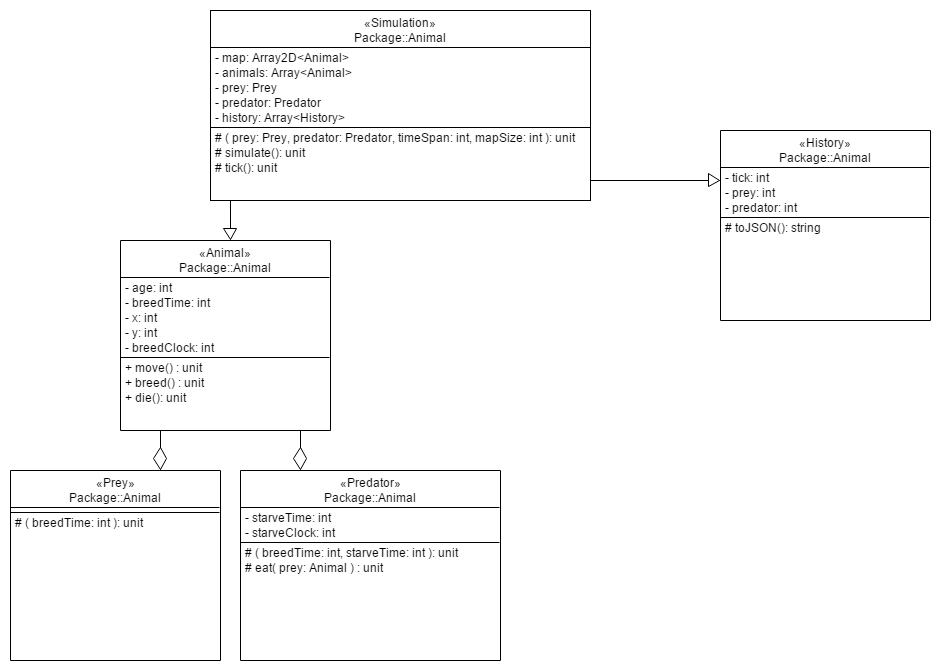
\includegraphics[width=520px]{figures/uml.png}

      \caption{UML diagram over vores klasse design}
      \label{fig:umlDiagram}
    \end{figure}

    Vi har haft flere overvejeler omkring det med starttilstand/indstillinger.
    Efter snakken frem og tilbage mellem kommandopropt-input og filbaseret input,
    er vi kommet frem til at bruge en fil.
    Det giver os den reneste kode og giver nem mulighed for at tilføje flere indstillinger.
    Filformatet for denne fil kunne være flere, både ".csv", ".txt" og "json" er gode formater,
    de to første er meget simple, mens ".json" er meget struktureret og det sikre en hvis datastruktur
    og mulighed for bedre error tjek. Derfor er valget faldet på ".json".

    Omkring output fil har vi også snakket om flere filformater,
    ".csv" er et meget bredt brugt format til simulationsdata,
    mens ".json" er nemt at læse ind fra. ".json" giver mest struktur,
    og afspejler også vores interne design og derfor faldt valget på det.

    \subsection*{Simulation}
      \texttt{Simulation} er den klasse der samler alt den nødvendige data for simulationen.
      Når en ny simulation skal begyndes, konstrueres et \texttt{Simulation} objekt,
      og til dets konstruktør funktion gives et settings objekt med de nødvendige indstillinger.
      Derefter sørger \texttt{Simulation} for at der bliver oprettet dyr,
      kørt ticks m.m.

    \subsection*{Animal}
      \texttt{Animal} er den globale/parent dyre klasse der som abstract klasse,
      ligger en standard for hvordan et dyr ser ud.
      Nogle få metoder kan implementeres på dette niveau, mens de fleste bare er abstract.

      \subsubsection*{Prey}
        \texttt{Prey} klassen nedarver fra den globale \texttt{Animal} klasse.
        Den skal bruges til at bestemme typen i listen/kortet over dyr,
        så \texttt{Prey} kan have en anden breedTime end Predators og så den kan implementere dens egen move.

      \subsubsection*{Predator}
        \texttt{Predator} klassen nedarver fra den globale \texttt{Animal} klasse,
        så udover de metoder og properties+fields der kommer derfra, skal den indeholde "starveTime"
        og "starveClock" for at holde styr på sult. For at kunne gøre det, skal den overskrive move metoden,
        og implementere end eat metode. En anden constructor skal også implementeres, fordi at kunne sætte de nye værdier.

    \subsection*{Settings} \label{ssec:designSettings}
      Typen \texttt{Settings} er et container element, 
      der indeholder starttilstanden for simulationen.
      Den giver en struktureret måde at gemme og tilgå de indstilliger der skal bruges.
      For at al logikken omkring indstillinger er indeholdt i en klasse,
      har vi valgt at klassen også selv loader en fil.

      Et Settings objekt kan derfor heller ikke oprettes uden at der gives en fil.

    \subsection*{HistoryRecord}
      HistoryRecord er en container klasse, der indeholder tilstanden for habitatet efter et tick.
      Den skal indeholde antal ticks siden start, antal preys og antal predators ved dette tick.
      Denne klasse ligger så struktur for et element i den JSON fil der gemmes når simulationen er slut.

  \section{Programbeskrivelse} \label{sec:programDescription}
    \begin{figure}[H]
      \centering
      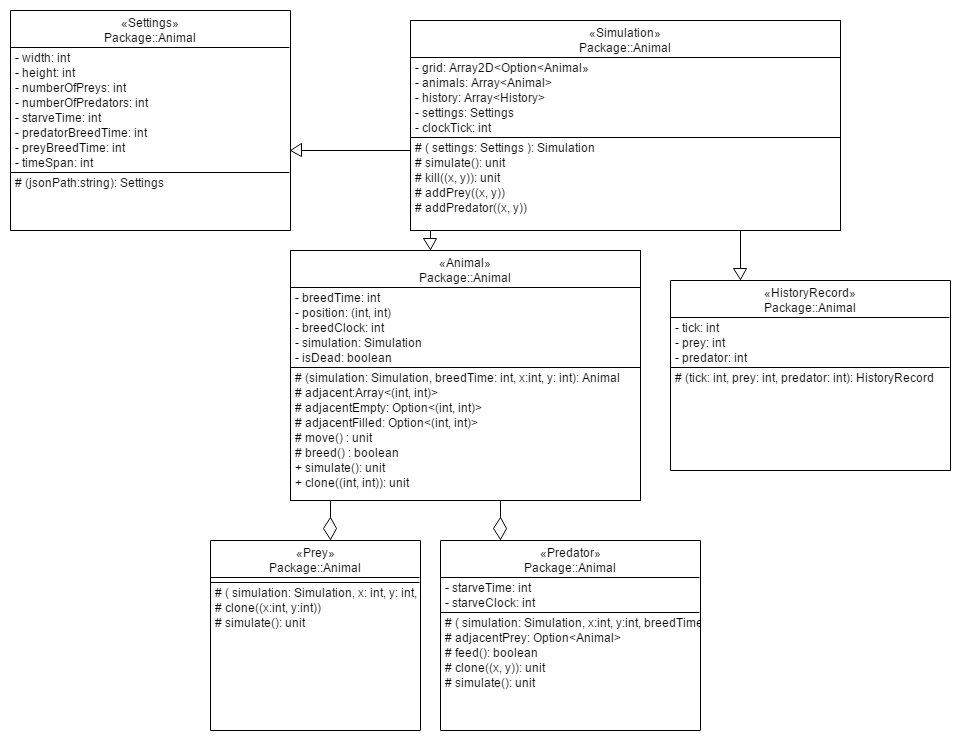
\includegraphics[width=520px]{figures/umlDone.png}
      \caption{UML diagram over vores færdige klasser}
      \label{fig:umlDiagramDone}
    \end{figure}

    \subsection*{Settings}
      Som tidligere beskrevet i \namedref{ssec:designSettings}, sættes simulationens indstillinger i en JSON fil,
      der vælges når programmet åbnes. Filerne ligges i mappen \path{/src/settings} og gemmes i JSON formatet,
      med fil extensionen ".json".
      Med programmet følger en default version, med et muligt testsenarie for programmet.
      Denne default fil kan ses i \namedref{lst:defaultSettings}.
      \lstinputlisting[language=JSON,caption={Default indstillinger},label={lst:defaultSettings}]{../src/settings/default.json}

      Filhåndteringen står \texttt{Settings} klassen for, og den gives med som parameter når en ny \texttt{Simulation} startes.
      De forskellige fields fra JSON filen loaded in i properties på \texttt{Settings} objektet.
      Filen kan loaded når \texttt{Settings} objektet oprettes, med det første parameter.
    
    \subsection*{Simulation}
    Simulation er en den klasse der styrer simulationen på den måde at den indeholder en matrix der indeholder
    alle de felter hvor dyrene kan befinde sig og en liste der indeholder alle dyrene selv, derudover er det
    Simulation der fortæller dyrene hvornår de kan foretage en handling. Simulation holder også styr på hvor
    langt inde i simulationen den er nået, og bestemmer dermed hvornår dyrene kan formere sig og hvornår
    rovdyrene sulter ihjel. Simulation indeholder følgende betydelige funktioner:

    \begin{itemize}
      \item simulate - kører igennem alle dyrene og lader dem udføre en enkel handling og opdaterer clockTick
      \item addPrey - laver et byttedyr på den givne position og med den givne breedTime
      \item addPredator - laver et rovdyr på den givne position, med den givne breedTime og den givne starveTime
    \end{itemize}
    
    \subsection*{Animal}
      Animal er en abstract-class, og er en skabelon for klasserne Prey og 
      Predator. 
    
    \subsection*{Prey}
      Prey implementere Animal klassen,
      den har to funktioner \lstinline$clone$ der opretter en ny prey
      og $simulate$ der køres ved hver tick.

      Simulate følger følgende rækkefølge, for operationerne,
      den kan kun gøre en af de tre følgende ved hvert tick.

      \begin{enumerate}
        \item isDead - Hvis den er markeret som død, gør ingenting
        \item breed - Hvis den kan føde, gør det
        \item move - Hvis den kan bevæge sig, gør det
      \end{enumerate}

    \subsection*{Predator}
      Predator implementere Animal klassen,
      den har fire funktioner \lstinline$clone$ der opretter en ny prey,
      $simulate$ der køres ved hver tick, $feed$ der prøver at spise
      og $adjacentPrey$ der prøver at finde en Prey i en nabocelle.

      Simulate følger følgende rækkefølge, for operationerne,
      den kan kun gøre en af de fire følgende ved hvert tick.

      Hvis dens starveTimer når nul, ved staten af et tick - så dør den.

      \begin{enumerate}
        \item isDead - Hvis den er markeret som død, gør ingenting
        \item feed - Hvis den kan spise en Prey i en af nabocellerne, gør det
        \item breed - Hvis den kan føde, gør det
        \item move - Hvis den kan bevæge sig, gør det
      \end{enumerate}
    
    \subsection*{HistoryRecord}
      HistoryRecord er implementeret som en klasse, der instantieres og derefter ikke kan ændres på.
      HistoryRecord har følgende fields:
      \begin{itemize}
        \item tick - Det clockTick tallene er fra
        \item prey - Antal preys ved dette clockTick
        \item predator - Antal predators ved dette clockTick
      \end{itemize}
      HistoryRecord har ved siden af det en metode, \lstinline$toJSON()$ der returnere en string.
      
  \section{Afprøvning} \label{sec:unitTest}

    Vi har lavet en del kørsler af vores simulation,
    med forskellige værdier.

    Her er vores default værdier.
    \lstinputlisting[language=JSON,caption={Default indstillinger},label={lst:defaultSettingsValues}]{../src/settings/default.json}

    Ovenstående værdier kan nedenstående, ved en af vores kørsler.
    Værdierne vil selvfølgelig varriere, fra kørsel til kørsel. Fordi vi har tilfældighed indblandet omkring bevægelsen.

    \begin{figure}[H]
      \centering
      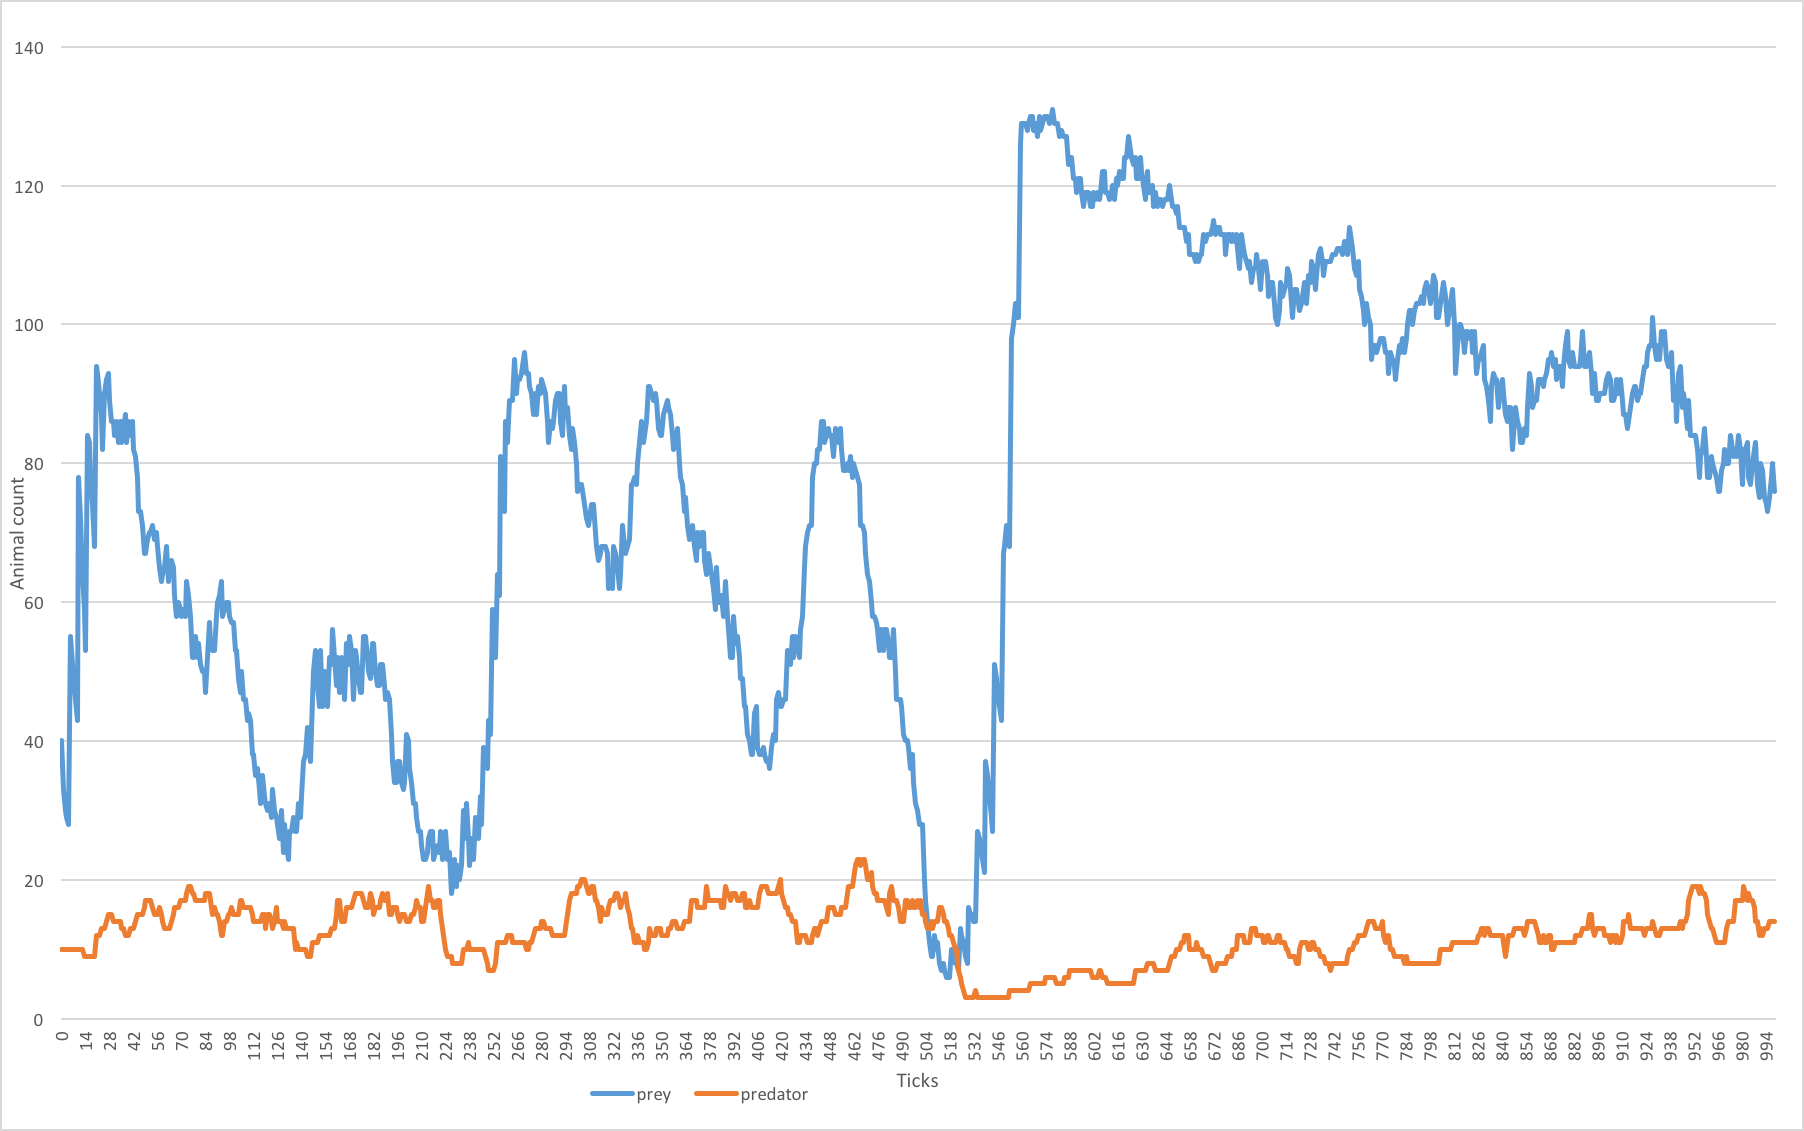
\includegraphics[width=400px]{figures/1sim.png}
      \caption{Graf over udviklingen for første simulation med "default.json"}
      \label{fig:firstSimulation}
    \end{figure}

    Vi har også testet med en setting, hvor der kommer mange prey's og en hvor der kommer mange predators.
    Her er først den setting, hvor det er bedst for prey's.
    \lstinputlisting[language=JSON,caption={Preys},label={lst:preysSettingsValues}]{../src/settings/prey.json}

    Den generere følgende graf.
    \begin{figure}[H]
      \centering
      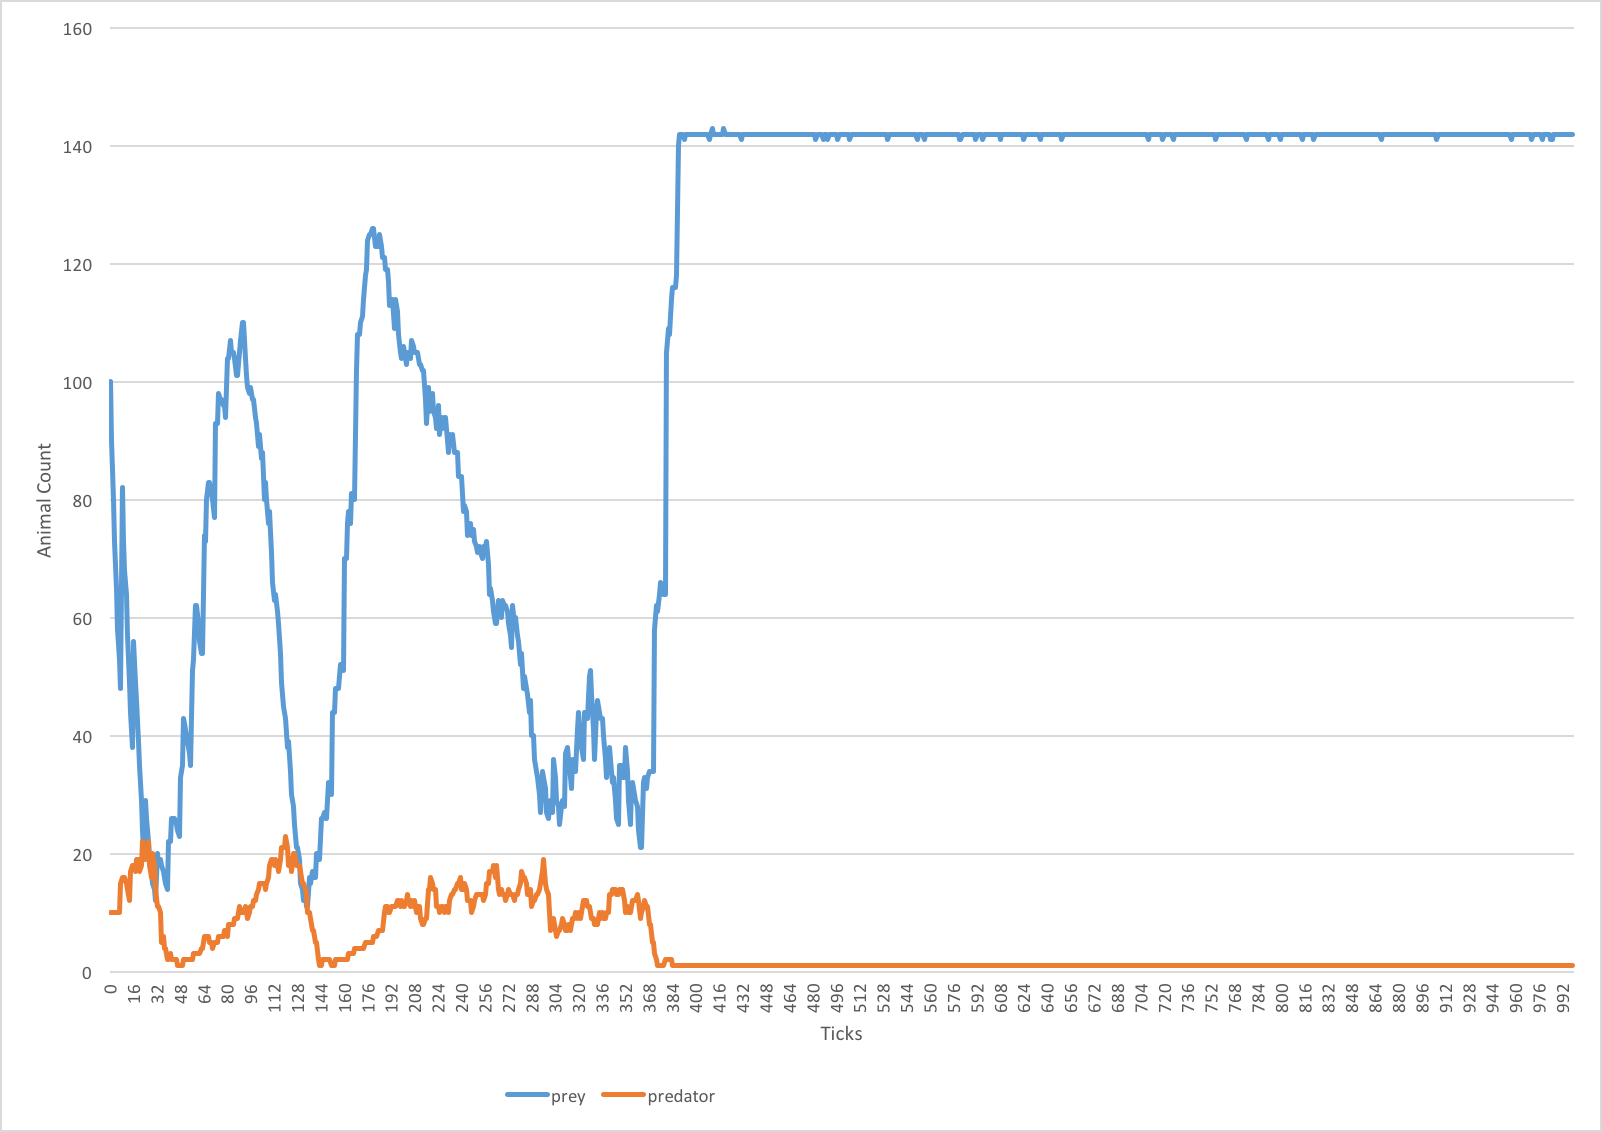
\includegraphics[width=400px]{figures/2sim.png}
      \caption{Graf over udviklingen for simulationen med "prey.json"}
      \label{fig:secondSimulation}
    \end{figure}

    Her er indstillingerne for den predator venlige version.
    \lstinputlisting[language=JSON,caption={Predators},label={lst:predatorSettingsValues}]{../src/settings/predator.json}

    Den generere følgende graf.
    \begin{figure}[H]
      \centering
      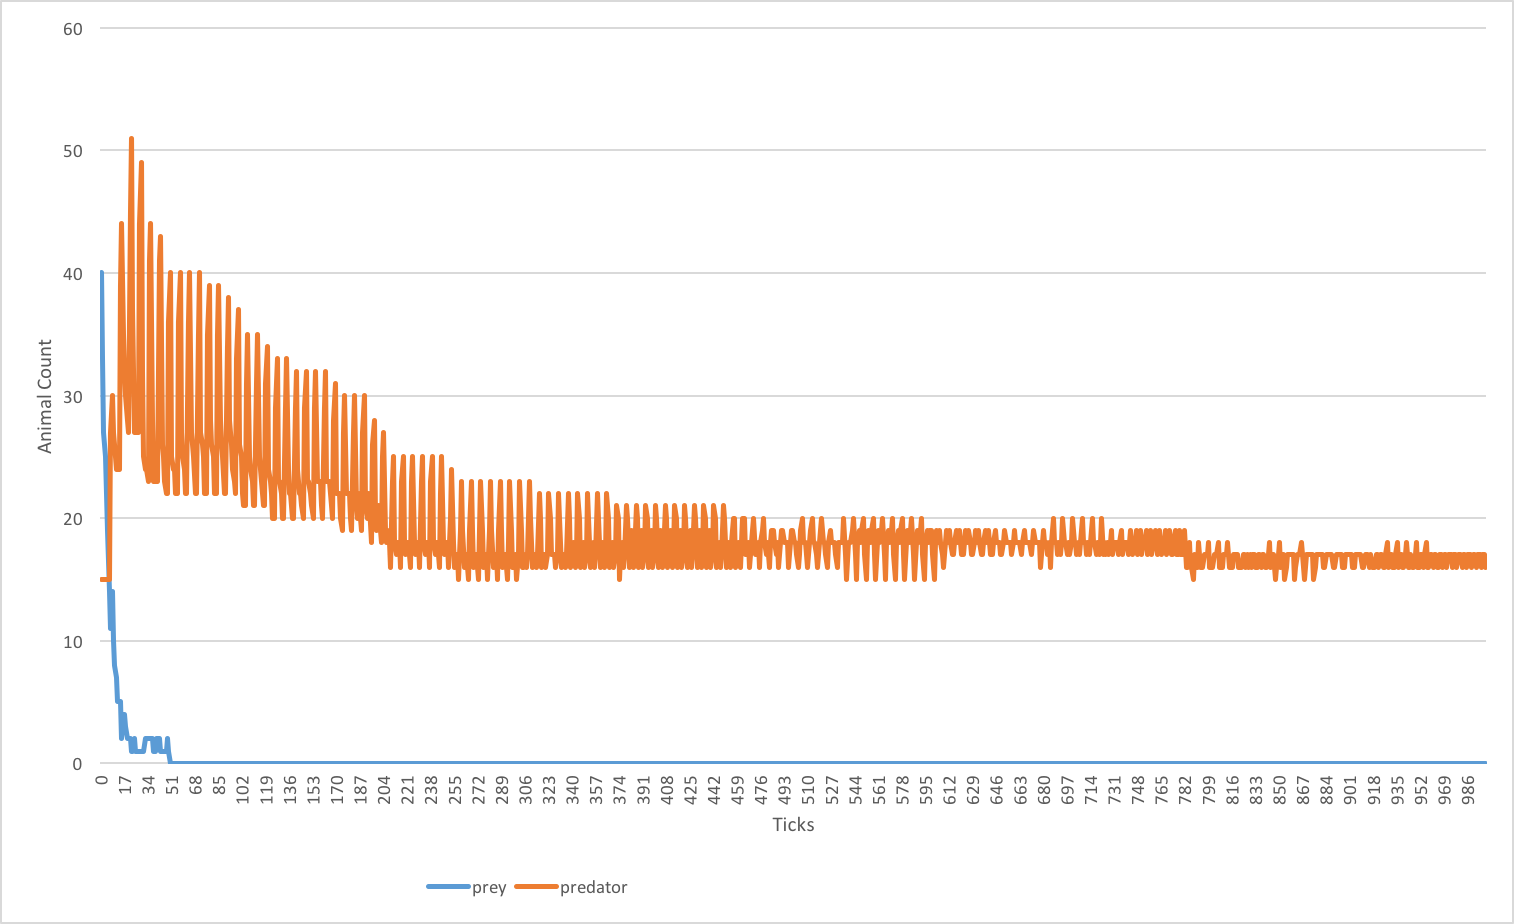
\includegraphics[width=400px]{figures/3sim.png}
      \caption{Graf over udviklingen for simulationen med "predator.json"}
      \label{fig:thirdSimulation}
    \end{figure}

	\section{Diskussion og konlusion} \label{sec:conclusion}
    Vi har i dette projektet designet og bygget en simulator,
    til at simulere hvordan to grupper af dyr "Prey" og "Predators" fungere i et naturligt habitat.
    Simulatoren er designet og udviklet efter OOP paradigmen, og udnytter klasser og nedarvning.
    Programmet lever op til de krav der er stillet til programmet i \namedref{ssec:demands}.
    Simulationen følger de stilne regler beskrevet under reglerne i \namedref{ssec:demands}.

    Programmet giver brugeren mulighed for selv at vælge starttilstand og 
    historien for simulationen gemmes i en struktureret fil, der er nem at læse.
    Programmet er designet med et UML diagram, og der er endda et UML diagram oer den færdige struktur.
    Programmet er kommenteret efter XML-kommentarstandarden og unit-testet.

  \section{Bilag}
     
      \subsection{Brugervejledning} \label{ssec:manual}
        
      \subsection{Kildekode} \label{ssec:sourceCode}
        \lstinputlisting[caption={Simulations klasser},label={lst:classes}]{../src/classes.fsx}
        \lstinputlisting[caption={Simulations klasser},label={lst:simulation}]{../src/simulation.fsx}
        \lstinputlisting[caption={Simulations klasser},label={lst:test}]{../src/test.fsx}
\end{document}